% natbib guide (https://gking.harvard.edu/files/natnotes2.pdf)
% \citet     #textual citations, print the abbreviated author list
% \citet*    #textual citations, print the full author list
% \citep     #parenthetical citations, print the abbreviated author list
% \citep*    #parenthetical citations, print the full author list
% \citealt    #the same as \citet but without any parentheses.
% \citealp    #the same as \citep but without any parentheses. 
% \citeauthor{ale91}         #Alex et al.
% \citeauthor*{ale91}        #Alex, Mathew, and Ravi
% \citeyear{ale91}           #1991 
% \citeyearpar{ale91}        #(1991)
\documentclass[english, xcolor=dvipsnames, aspectratio=169]{beamer}

% Text encoding
\usepackage[english]{babel}

% Justify text (package and function)
% \apptocmd{command}{code}{success}{failure}
\usepackage{ragged2e}
\apptocmd{\frame}{}{\justifying}{} 
% Justify text in \item
\newcommand{\itemj}{\item \justifying}

% If...else package
\usepackage{ifthen}

% Package to set transparent background image
\usepackage{tikz}

% Include image package
\usepackage{graphicx}
% Set default path for images
\graphicspath{ {./imgs/} }
% Set figure number when included
\setbeamertemplate{caption}[numbered]

% Bibliography packages
\usepackage[sort, round]{natbib}

% roman number
\usepackage{romannum}

\usepackage{amsmath}
%code settings
\usepackage{listings}
\usepackage{color}
\definecolor{dkgreen}{rgb}{0,0.6,0}
\definecolor{gray}{rgb}{0.5,0.5,0.5}
\definecolor{mauve}{rgb}{0.58,0,0.82}

\lstdefinestyle{Python}{% myPython是格式的名字
	frame=tb,
	language=Python,
	aboveskip=3mm,
	belowskip=3mm,
	showstringspaces=false,
	columns=flexible,
	numberstyle=\small\color{red},
	basicstyle={\small\ttfamily},
	keywordstyle=\color{blue},
	commentstyle=\color{dkgreen},
	stringstyle=\color{mauve},
	breaklines=True,
	breakatwhitespace=False,
	tabsize=3
}
%------------------------算法(伪代码)的环境设置---------------------------------------------- 
\usepackage{algorithm,algpseudocode,float}
%\usepackage{algorithmic}
\usepackage{lipsum}
%\renewcommand{\algorithmicrequire}{\textbf{input:}}   % Use Input in the format of Algorithm  
%\renewcommand{\algorithmicensure}{\textbf{process:}}    % Use Output in the format of Algorithm
\floatname{algorithm}{Pseudocode}  
\renewcommand{\algorithmicrequire}{\textbf{}}  
\renewcommand{\algorithmicensure}{\textbf{}} 
\makeatletter
\newenvironment{breakablealgorithm}
  {% \begin{breakablealgorithm}
   \begin{center}
     \refstepcounter{algorithm}% New algorithm
     \hrule height.8pt depth0pt \kern2pt% \@fs@pre for \@fs@ruled
     \renewcommand{\caption}[2][\relax]{% Make a new \caption
       {\raggedright\textbf{\ALG@name~\thealgorithm} ##2\par}%
       \ifx\relax##1\relax % #1 is \relax
         \addcontentsline{loa}{algorithm}{\protect\numberline{\thealgorithm}##2}%
       \else % #1 is not \relax
         \addcontentsline{loa}{algorithm}{\protect\numberline{\thealgorithm}##1}%
       \fi
       \kern2pt\hrule\kern2pt
     }
  }{% \end{breakablealgorithm}
     \kern2pt\hrule\relax% \@fs@post for \@fs@ruled
   \end{center}
  }

%%%%%%%%%%%%%%%%%%%%%%%%%%%%%%%%%%%%%%%%%%%%%%%%%%%%%%%%%%%%

% Define colors variables
\definecolor{red}{rgb}{0.631, 0.094, 0.094} % primary color
\definecolor{grey}{rgb}{0.3686, 0.5255, 0.6235} % secondary color
\xdefinecolor{tsinghua}{rgb}{0.455,0.204,0.506}
% Set theme palette colors

\setbeamercolor{palette primary}{bg=tsinghua,fg=white}
\setbeamercolor{palette secondary}{bg=tsinghua,fg=white}
\setbeamercolor{palette tertiary}{bg=tsinghua,fg=white}
\setbeamercolor{palette quaternary}{bg=tsinghua,fg=white}
% strucure means itemize, enumerate, etc
\setbeamercolor{structure}{fg=black} 

% Set bibliography colors
\setbeamercolor{bibliography item}{fg=red}
\setbeamercolor{bibliography entry author}{fg=black}
\setbeamercolor{bibliography entry title}{fg=black}
\setbeamercolor{bibliography entry location}{fg=black}
\setbeamercolor{bibliography entry note}{fg=black}
% Replaces book icon in bibliography with enumeration
\setbeamertemplate{bibliography item}{[\theenumiv]}

% Table of contents style
% \setbeamertemplate{section in toc}[sections numbered]
% \setbeamertemplate{subsection in toc}[subsections numbered]

% \setbeamertemplate{section in toc}[circle]
% \setbeamertemplate{subsection in toc}[ball unnumbered]
\setbeamertemplate{section in toc}[circle]
\setbeamertemplate{subsection in toc}[ball unnumbered]
\setbeamercolor*{item projected}{fg=white,bg=tsinghua}
\useinnertheme{circles}

\setbeamertemplate{navigation symbols}{}
\setbeamertemplate{bibliography item}[text]
\setbeamertemplate{caption}[numbered]
% Header with navigation bar
\setbeamertemplate{headline}
{
    \leavevmode
    \hbox{
    \begin{beamercolorbox}[wd=\paperwidth,ht=2.5ex,dp=1.125ex]{palette quaternary}
    \insertsectionnavigationhorizontal{\paperwidth}{}{\hskip0pt plus1filll}
    \end{beamercolorbox} 
    }
}
% Footer with custom caption
\setbeamertemplate{footline}
{
    \leavevmode
    \hbox{
    \begin{beamercolorbox}[wd=.33\paperwidth,ht=2.6ex,dp=1ex,center]{palette quaternary}
    \usebeamerfont{author in head/foot}\insertshortauthor\hspace*{1ex}
    \end{beamercolorbox}
    \begin{beamercolorbox}[wd=.33\paperwidth,ht=2.6ex,dp=1ex,center]{palette quaternary}
    \usebeamerfont{institute in head/foot}\insertshortinstitute
    \end{beamercolorbox}
    \begin{beamercolorbox}[wd=.33\paperwidth,ht=2.6ex,dp=1ex,center]{palette quaternary}
    \insertframenumber{} / \inserttotalframenumber
    \end{beamercolorbox}}
    \vskip0pt
}

% Global Background must be put in preamble

% \usebackgroundtemplate
% {
%     \tikz\node[opacity=0.3]{
\includegraphics[height=\paperheight, width=\paperwidth]{background.png}};
% }

% One line command to print table of contents - two parameters for modes
\newcommand{\customToC}[2]
{
    \begin{frame}{Overview}
    \tableofcontents[#1,#2]
    \end{frame}
}
% Command to plot centered figure
% Parameters: #1=image name, #2=caption 
\newcommand{\includefigure}[2]
{
    \begin{figure}[h]
    \caption{#2}
    \centering
    \includegraphics[width=0.5\textwidth]{#1}
    \end{figure}
}
% Command to set section name as variable (\renewcommand to update)
\newcommand{\sectiontitle}{}
% Command to set subsection name as variable (\renewcommand to update)
\newcommand{\subsectiontitle}{}
%*************************************************************************
% Body paragraph 正文部分
%*************************************************************************
\begin{document}
% Title page
\titlegraphic{
\includegraphics[height=2cm]{sigs.png}}
\title{Group Meeting Report \Romannum{2}}
\subtitle{Implementation Details of Proximal Policy Optimization}
\author{LongX.He}
\institute{Tsinghua ShenZhen International Graduate School}
% Date
\day=15\relax
\month=05\relax
\year=2022\relax

\frame{\titlepage}
% Complete table of contents (ToC)
% \customToC{hideallsubsections}{}
\customToC{}{}

% Section name and highlighted ToC

\section{Proximal Policy Optimization}
% \customToC{currentsection,hideothersubsections}{}


% Section name and highlighted ToC

\subsection{PPO Penalty}
\begin{frame}{PPO Penalty}
 \begin{itemize}
        \item Use penalty instead of constraint \cite{schulman_proximal_2017}  :
                 $$ \max_{\theta} \ \hat{\mathbb{E}_{t}}\left[\frac{\pi_{\theta}(a_t|s_t)}{\pi_{\theta_{old}(a_t|s_t)}}\hat{A_t}\right]-C\cdot\overline{KL}_{\pi_{\theta_{old}}}(\pi_{\theta})
         $$
         \item Pseudocode
             \begin{algorithm}[H]  
  \caption{PPO Penalty}  
  \begin{algorithmic}[1] 
    \For{iteration=1,2,...}
    \State Run policy for T timesteps  or N tragectories
    \State Estimate advantage function at all timesteps
    \State Do SGD on above objective for some number of epochs
    \State If KL too high,increase $\beta$. If KL too low,decrease $\beta$
    
    \EndFor   
  \end{algorithmic}  
\end{algorithm}

\end{itemize}

\end{frame}

\subsection{PPO-Clip}
\begin{frame}{PPO-Clip}
\begin{itemize}
    \item PPO-Clip:
    $$\theta=argmax_{\theta} \ \hat{\mathbb{E}_{s}}\left[\min\left(\frac{\pi_{\theta}(a_t|s_t)}{\pi_{\theta_{old}(a_t|s_t)}}\hat{A_t},clip\left(\frac{\pi_{\theta}(a_t|s_t)}{\pi_{\theta_{old}(a_t|s_t)}},1-\epsilon,1+\epsilon\right)\hat{A_t}\right)\right]
$$
\item GAE $where \ \delta_{t+l}=r_{t+l}+\gamma V(S_{t+l+1})-V(S_{t+l})$:
\begin{equation*}
    \begin{aligned}
            A_{t}^{GAE} &= (1-\lambda)(A_{t}^{1}+\lambda A_{t}^{2}+\lambda A_{t}^{3} + \dots)\\
               &= (1-\lambda)(\delta_t + \lambda(\delta_t+\gamma\delta_{t+1})+\lambda^2(\delta_t+\gamma\delta_{t+1}+\gamma^2\delta_{t+2})+\dots)\\
               &= (1-\lambda)(\delta_t(1+\lambda+\lambda^2+\dots)+\gamma\delta_{t+1}(\lambda+\lambda^2+\lambda^3+\dots)+\dots)\\
               &= (1-\lambda)\left(\delta_t\frac{1}{1-\lambda}+\gamma\delta_{t+1}\frac{\lambda}{1-\lambda}+\lambda^2\delta_{t+2}\frac{\lambda^2}{1-\lambda}+\dots\right)\\
               &= \sum_{l=0}^{\infty}(\gamma\lambda)^l\delta_{t+l} 
    \end{aligned}
\end{equation*}

% \gamma^2\delta_{t+2}(\lambda^2+\lambda^3+\lambda^4+\dots)+



    
\end{itemize}


\end{frame}









%*************************************************************************
%*************************************************************************
%*************************************************************************

\section{Implementation Details}
% \customToC{currentsection,hideothersubsections}{}


% Section name and highlighted ToC

\subsection{Envs Details}
\begin{frame}{Envs Details(\citet{blog})}
\begin{itemize}
        \item Vectorized architecture
        \begin{itemize}
            \item  PPO leverages an efficient paradigm known as the vectorized architecture that features a single learner that collects samples and learns from multiple environments.
        \end{itemize}
    \item Handling of action clipping to valid range and storage
        \begin{itemize}
    \item After a continuous action is sampled, such action could be invalid because it could exceed the valid range of continuous actions in the environment. To avoid this, add applies the rapper to clip the action into the valid range.
    
    \end{itemize}
    
    
    \item Normalization of Observation
    \begin{itemize}
        \item     At each timestep, the VecNormalize wrapper preprocesses the observation before feeding it to the PPO agent. The raw observation was normalized by subtracting its running mean and divided by its variance.
    \end{itemize}

    \item Observation Clipping
    \begin{itemize}
        \item     Followed by the normalization of observation, the normalized observation is further clipped by VecNormalize to a range.
    \end{itemize}

\end{itemize}

\end{frame}

\begin{frame}{Envs Details(\citet{blog})}
\begin{itemize}
        \item Reward Scaling
        \begin{itemize}
            \item The VecNormalize also applies a certain discount-based scaling scheme, where the rewards are divided by the standard deviation of a rolling discounted sum of the rewards (without subtracting and re-adding the mean).
            \item Engstrom, Ilyas, et al., (2020) reported that reward scaling can significantly affect the performance of the algorithm and recommends the use of reward scaling.
        \end{itemize}
        
        \item Reward Clipping 
        \begin{itemize}
            \item Followed by the scaling of reward, the scaled reward is further clipped by VecNormalize to a range.
\item A similar approach can be found in (Mnih et al., 2015). There is currently no clear evidence that Reward Clipping after Reward Scaling can help with learning.
        \end{itemize}
\end{itemize}

\end{frame}



% \begin{frame}{}
% \lstinputlisting[style=Python]{code/env.py}
    
% \end{frame}

\subsection{Net Detail}
 \begin{frame}{Net Detail(\citet{blog})}
\begin{itemize}
    \item Orthogonal Initialization of Weights and Constant Initialization of biases
    \item The Adam Optimizer’s Epsilon Parameter 
    \item Adam Learning Rate Annealing
    \item Mini-batch Updates
    \item Normalization of Advantages
    \item Value Function Loss Clipping
    \item Overall Loss and Entropy Bonus*
    \begin{itemize}
        \item    Andrychowicz, et al. (2021) overall find no evidence that the entropy term improves performance on continuous control environments.
    \end{itemize}
    
 

    % \item  \lstinputlisting[style=Python]{code/ini.py}
    % \item   \lstinputlisting[style=Python]{code/adam.py}

\end{itemize}


 \end{frame}

 \begin{frame}{Net Detail(\citet{blog})}
\begin{itemize}

    % \item  \lstinputlisting[style=Python]{code/ini.py}
    % \item   \lstinputlisting[style=Python]{code/adam.py}
    \item Global Gradient Clipping
    \item Shared and separate MLP networks for policy and value functions
    \item Continuous actions via normal distributions
    \item State-independent log standard deviation 
    \item Independent action components 
    \begin{itemize}
        \item Although our intuition tells us that there may be dependencies between action choices in different dimensions of policies in some environments, what is the optimal choice is still an open question.
    \end{itemize}
 
\end{itemize}


 \end{frame}






%*************************************************************************
%*************************************************************************
%*************************************************************************

\section{Experiments }
% \customToC{currentsection,hideothersubsections}{}

% Section name and highlighted ToC
\subsection{Experiments Environments}
\begin{frame}{Experiments Environments}
\begin{itemize}
    \item HalfCheetahBulletEnv-v0
    \begin{itemize}
    \item The goal is to apply a torque
    on the joints to make the cheetah run forward (right) as fast as possible,
    with a positive reward allocated based on the distance moved forward and a
    negative reward allocated for moving backward. The torso and head of the
    cheetah are fixed, and the torque can only be applied on the other 6 joints
    over the front and back thighs (connecting to the torso), shins
    (connecting to the thighs) and feet (connecting to the shins).
        \item  The action space is a Box(-1, 1, (6,), float32). An action represents the torques applied between *links*.
        \item  Observations consist of positional values of different body parts of the
    cheetah, followed by the velocities of those individual parts (their derivatives) with all the positions ordered before all the velocities.
    By default, the observation is a ndarray with shape (17,).
    \item The reward consists of two parts:*forward reward*, *ctrl cost*.
    \end{itemize}
    
\end{itemize}
\end{frame}

\begin{frame}{Experiments Environments}
\begin{itemize}
    \item Humanoid-v3
    \begin{itemize}
    \item This environment is based on the environment introduced by Tassa, Erez and Todorov
    in ["Synthesis and stabilization of complex behaviors through online trajectory optimization"](https://ieeexplore.ieee.org/document/6386025).
    The 3D bipedal robot is designed to simulate a human. It has a torso (abdomen) with a pair of
    legs and arms. The legs each consist of two links, and so the arms (representing the knees and
    elbows respectively). The goal of the environment is to walk forward as fast as possible without falling over.

        \item   The action space is a Box(-1, 1, (17,), float32). An action represents the torques applied at the hinge joints.
        \item    Observations consist of positional values of different body parts of the Humanoid,
     followed by the velocities of those individual parts (their derivatives) with all the
     positions ordered before all the velocities.By default, the observation is a ndarray with shape (376,) .
    \item The reward consists of three parts:*forward reward; *ctrl cost*;*contact cost 
    \end{itemize}
    
\end{itemize}
\end{frame}




\subsection{HalfCheetahBulletEnv-v0}

\begin{frame}{HalfCheetahBulletEnv-v0}
    \begin{figure}[ht]
        \begin{minipage}[b]{0.32\linewidth}
            \centering
            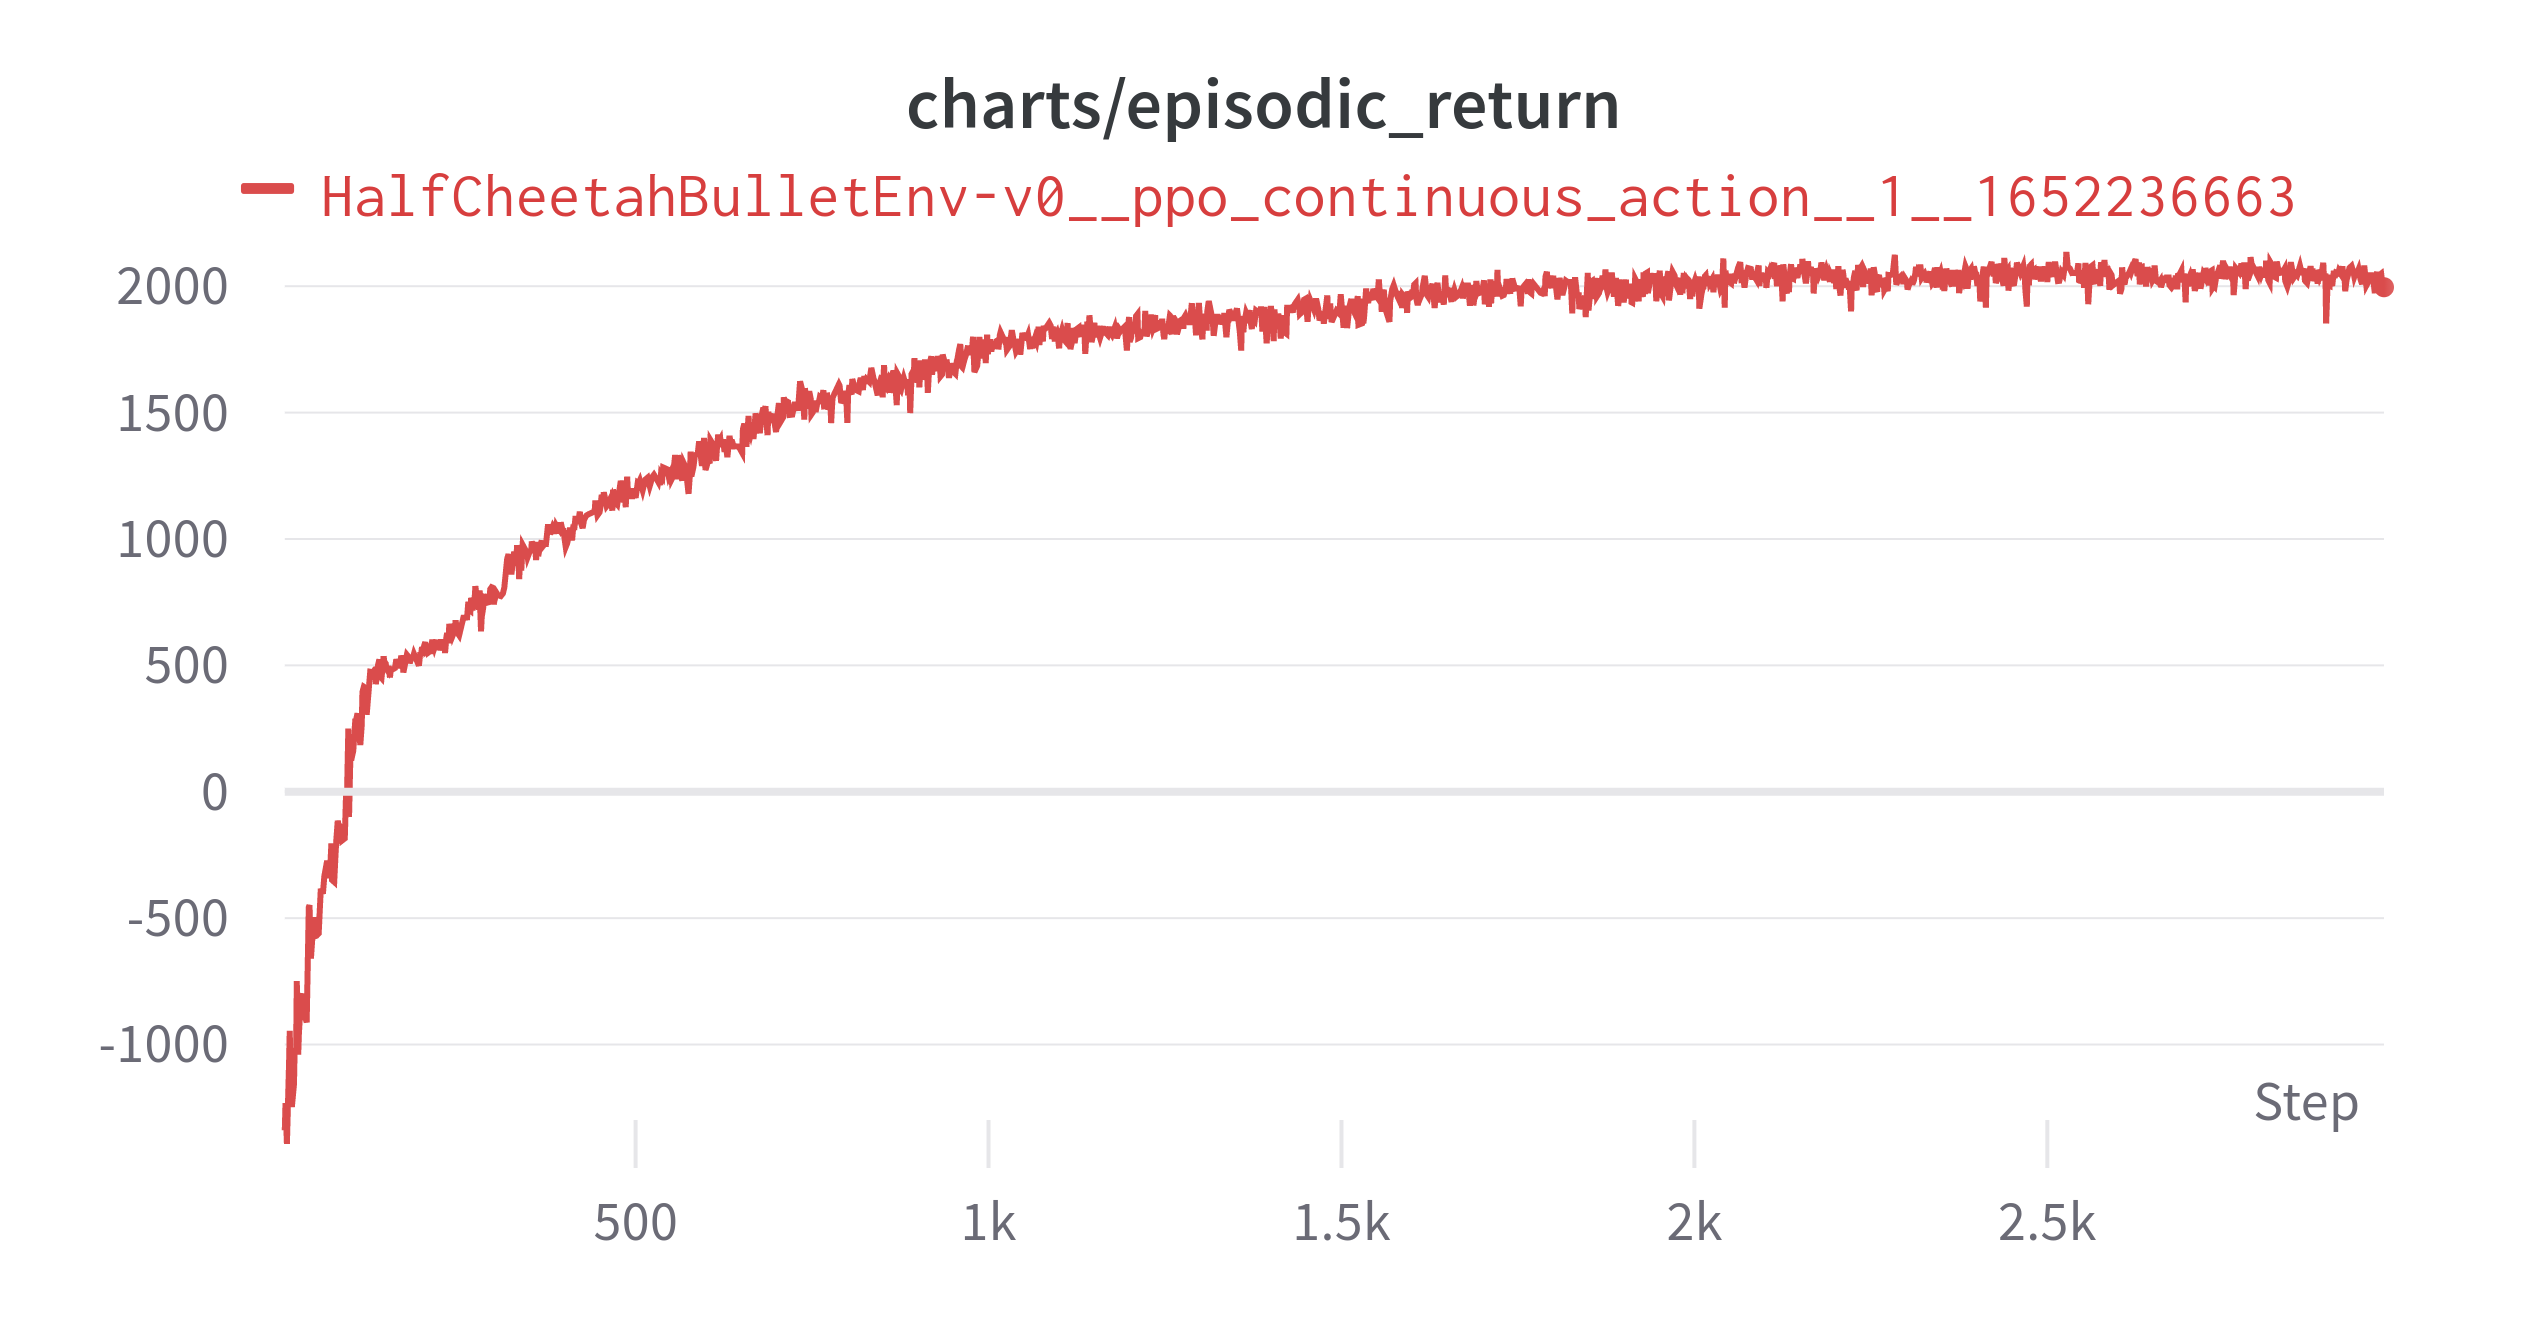
\includegraphics[width=\textwidth]{half_.png}
            \caption{Reward on HalfCheetahBulletEnv-v0}
            \label{fig:cifar10}
        \end{minipage}
        \hspace{0.5cm}
        \begin{minipage}[b]{0.32\linewidth}
            \centering
            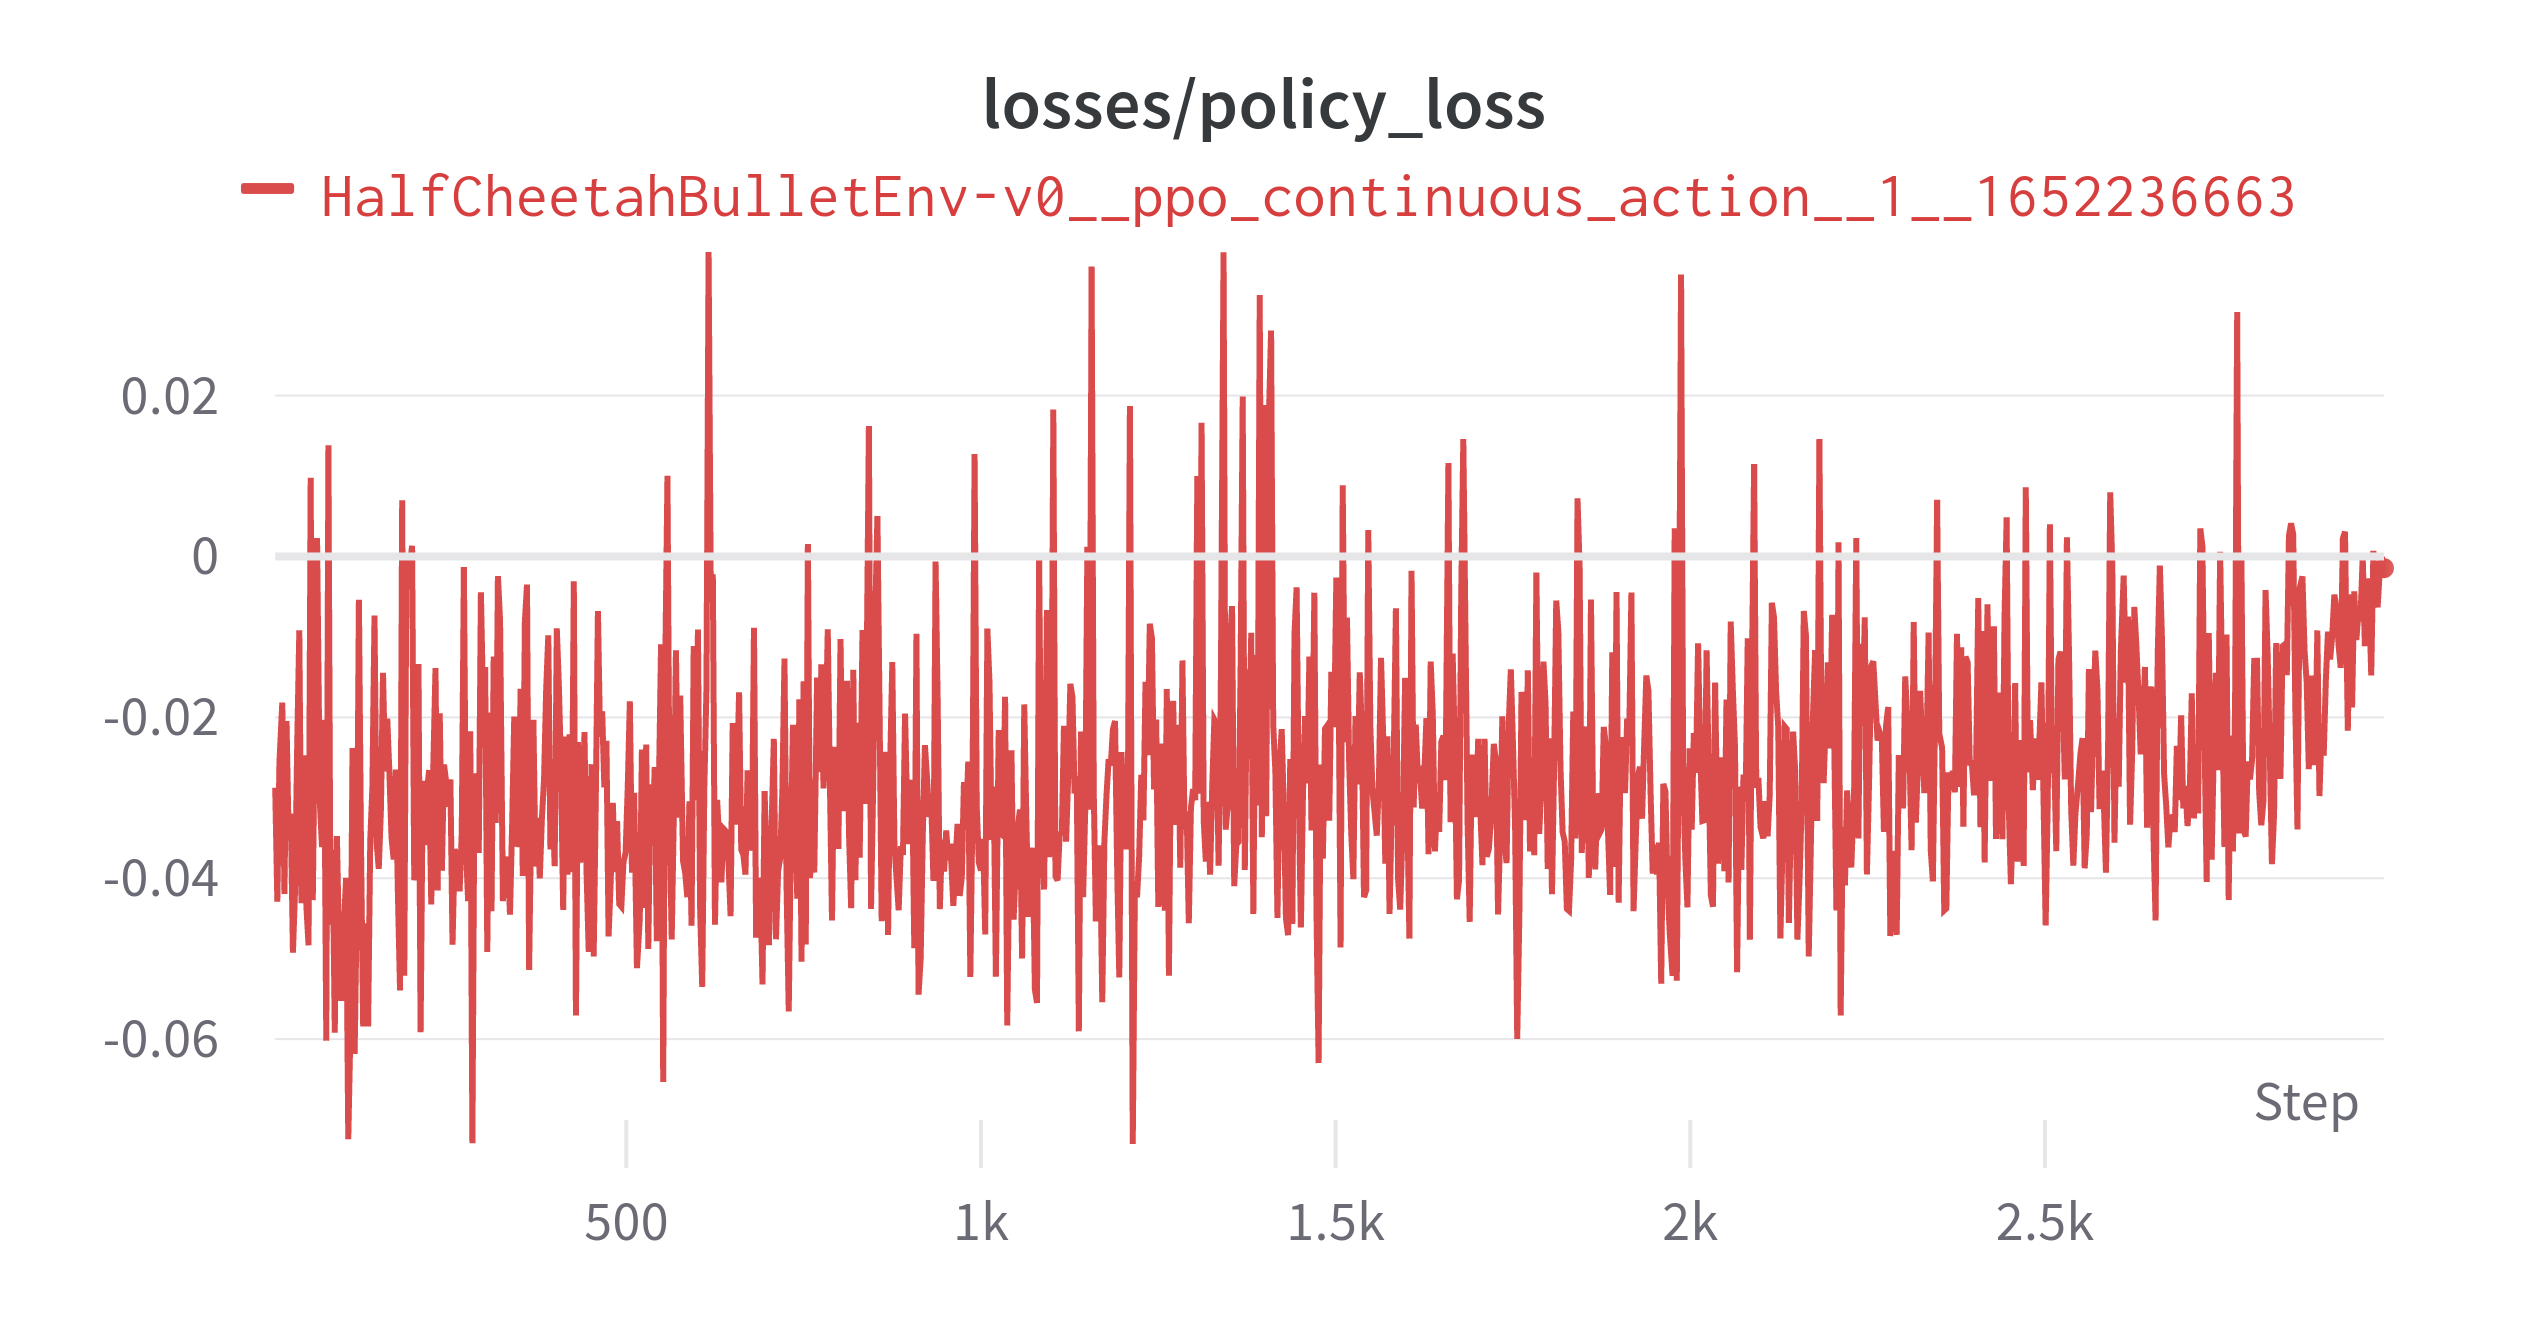
\includegraphics[width=\textwidth]{half_policy_loss.png}
            \caption{Policy loss on HalfCheetahBulletEnv-v0}
            \label{fig:cifar100}
        \end{minipage}
        \begin{minipage}[b]{0.32\linewidth}
            \centering
            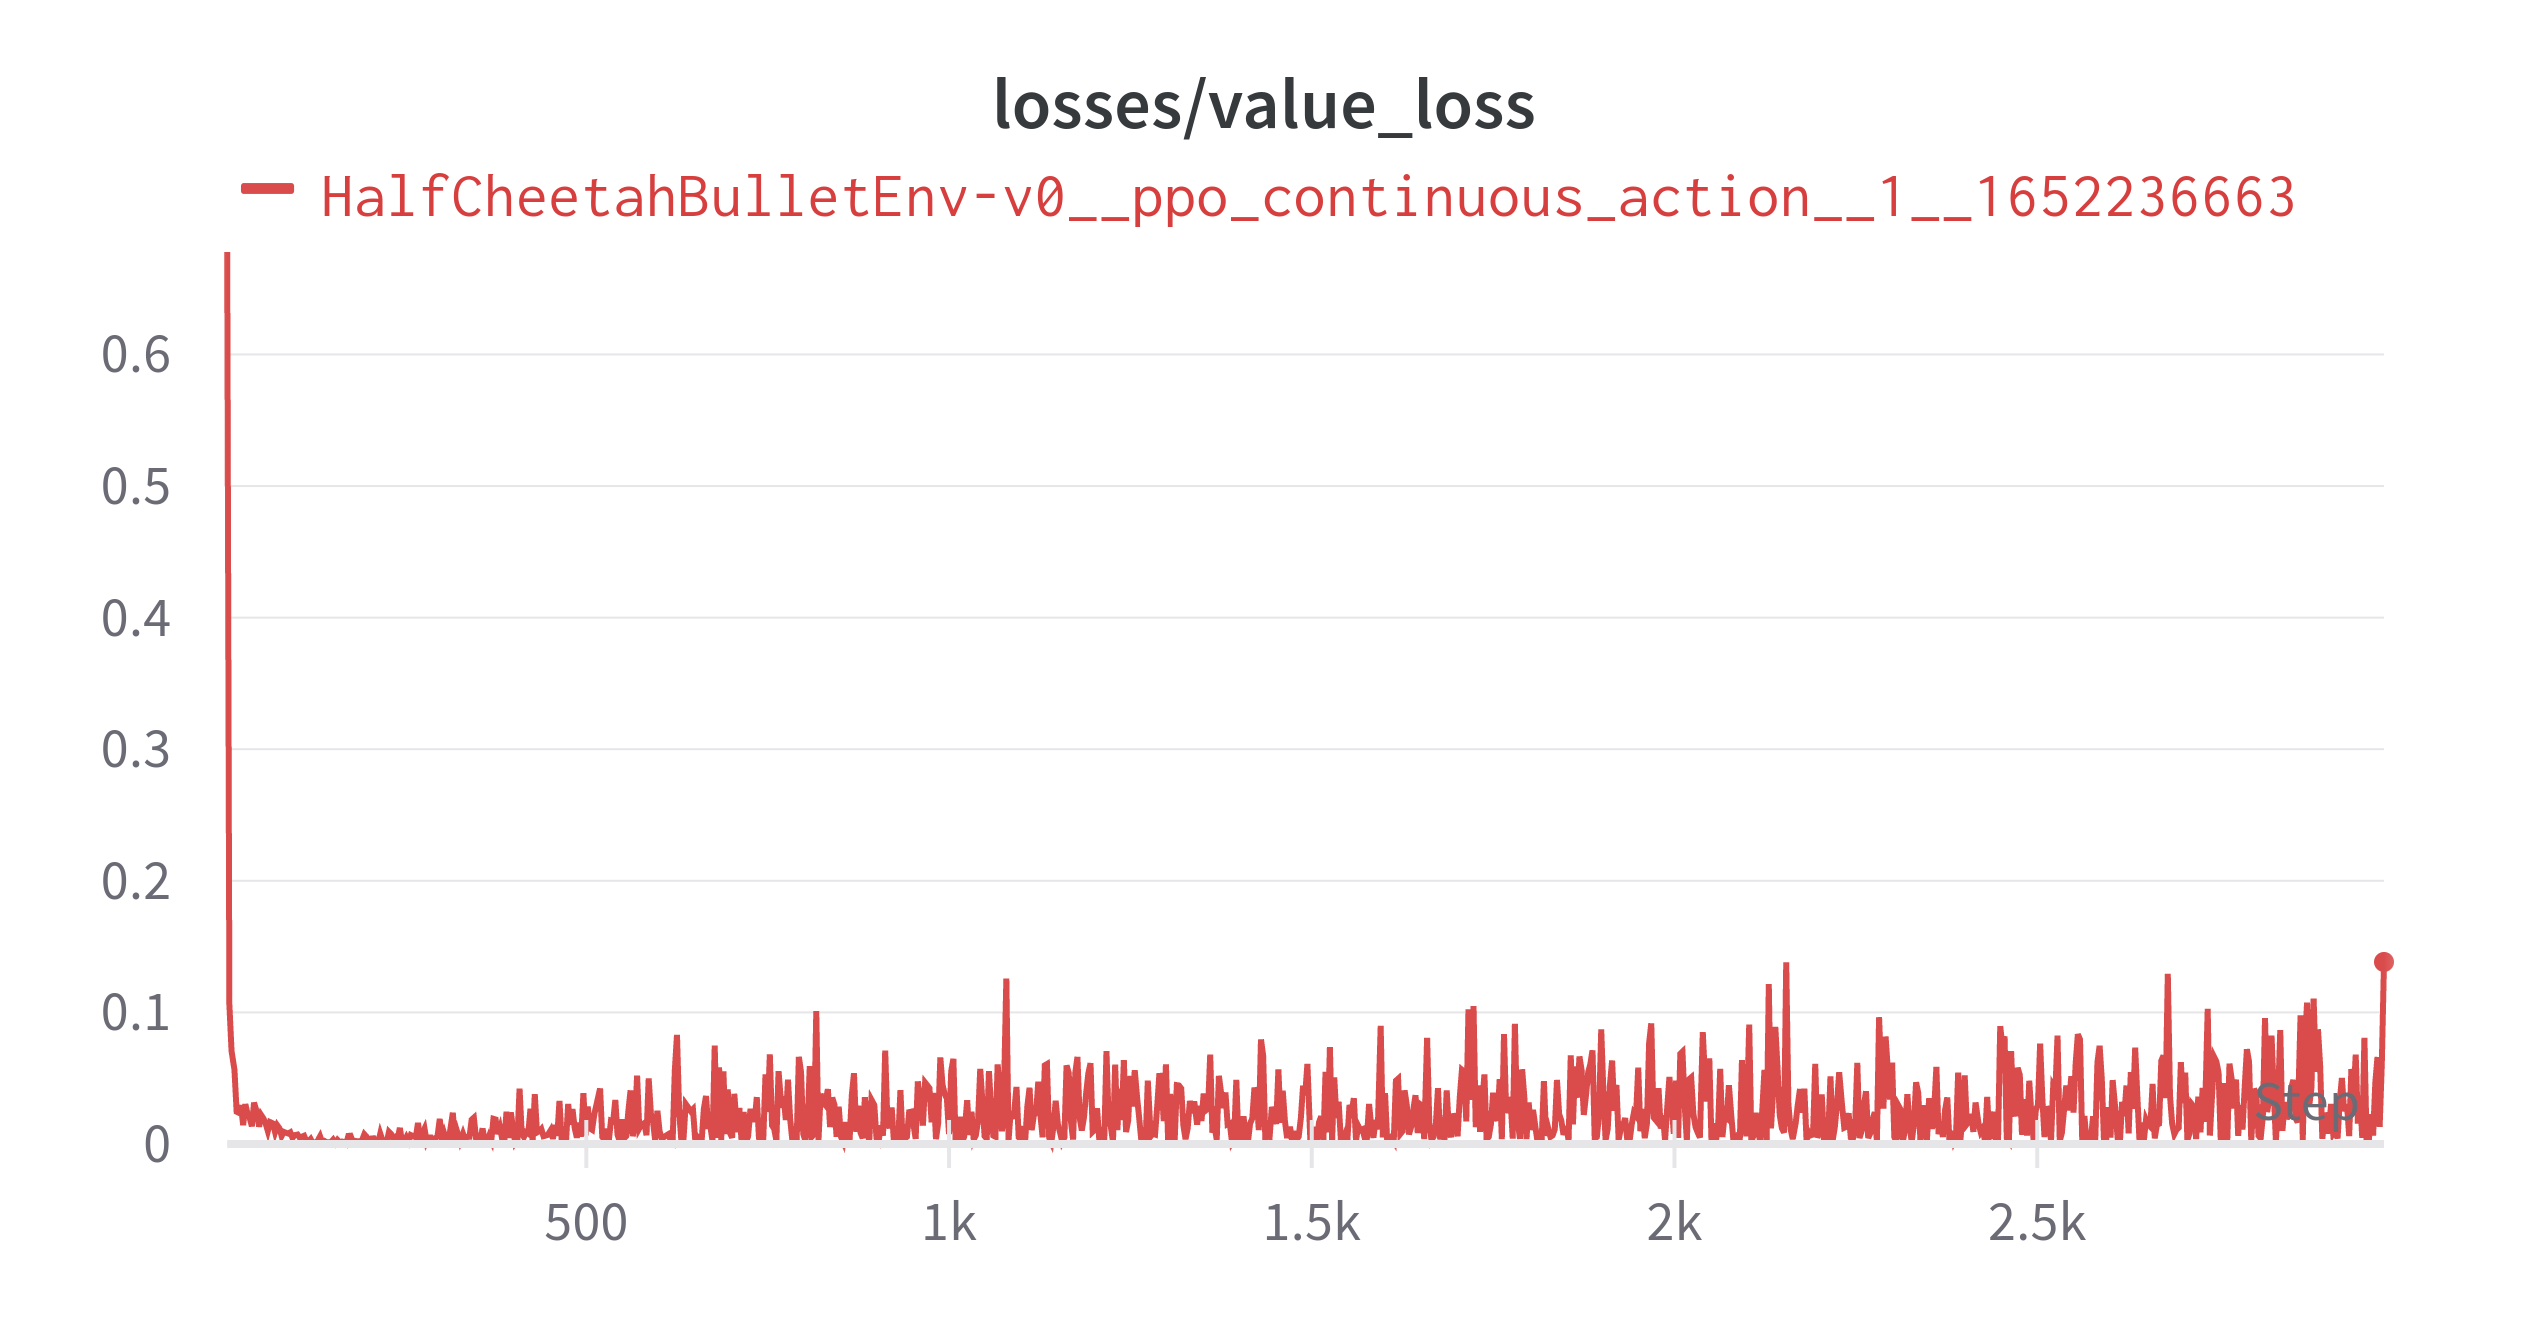
\includegraphics[width=\textwidth]{half_value_loss.png}
            \caption{Value loss on HalfCheetahBulletEnv-v0}
            \label{fig:imagenet1k}
        \end{minipage}
    \end{figure}


\end{frame}

% Section name and highlighted ToC

\subsection{Humanoid-v3}
% \customToC{currentsection,hideothersubsections}{}

% Slide with four figures
\begin{frame}{Humanoid-v3}
    \begin{figure}[ht]
        \begin{minipage}[b]{0.32\linewidth}
            \centering
            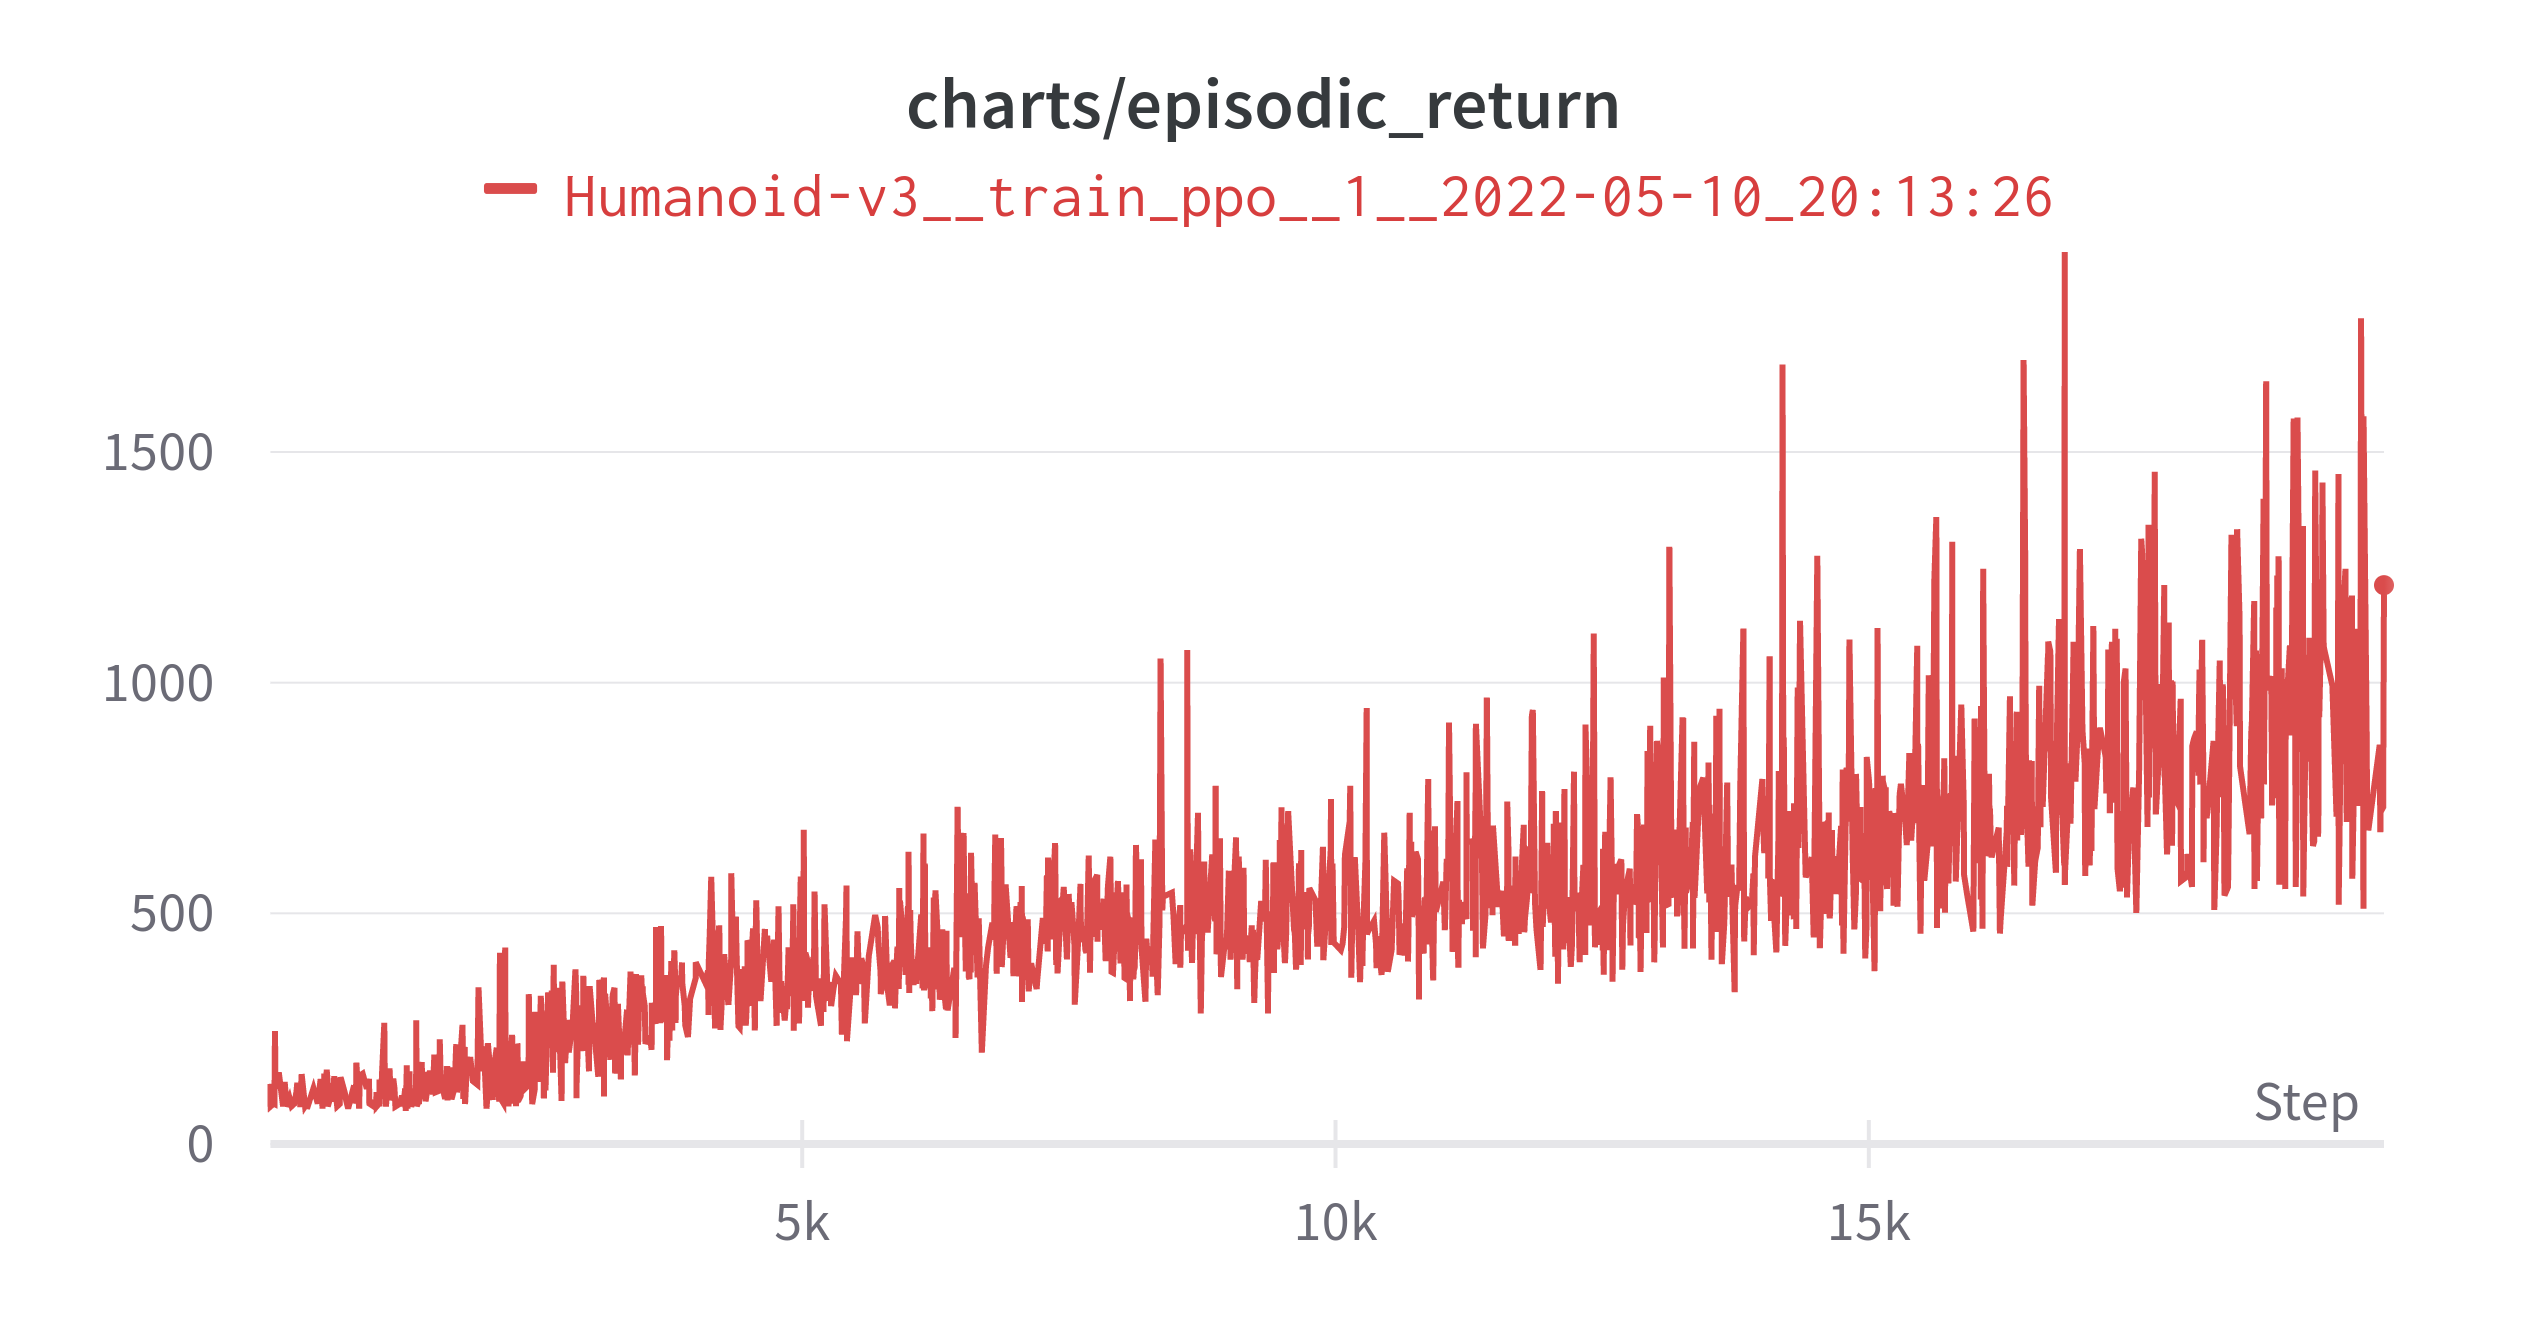
\includegraphics[width=\textwidth]{humanoid_.png}
            \caption{Reward on Humanoid-v3}
            \label{fig:cifar10}
        \end{minipage}
        \hspace{0.5cm}
        \begin{minipage}[b]{0.32\linewidth}
            \centering
            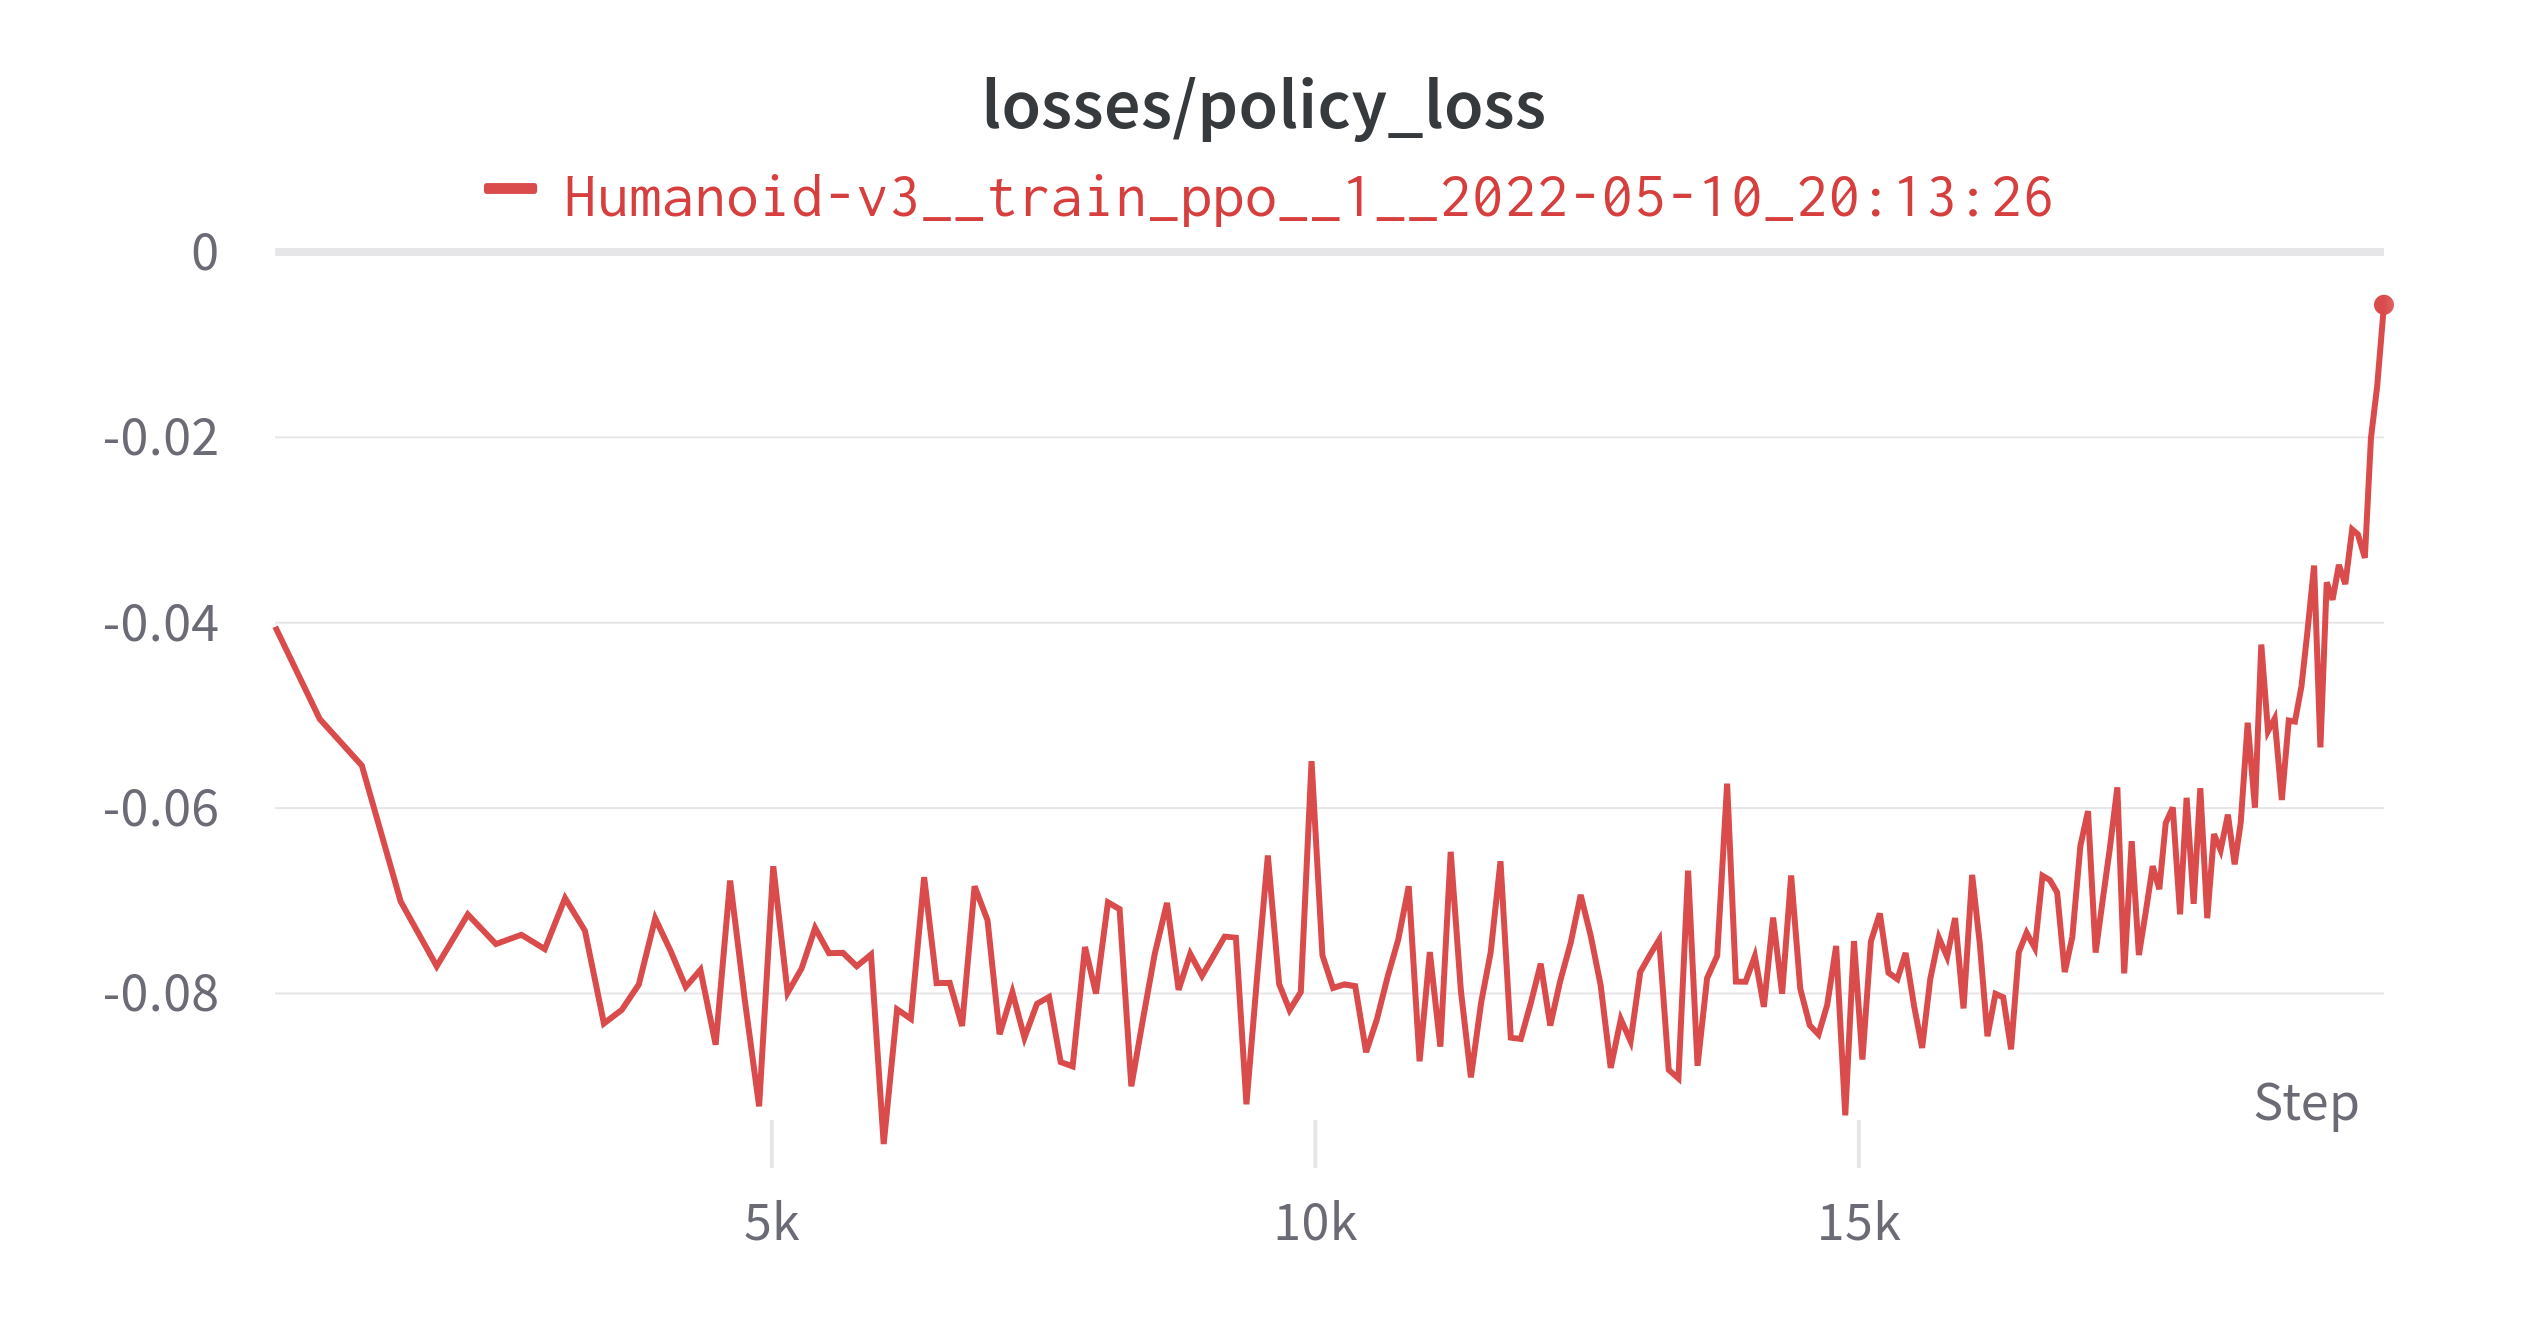
\includegraphics[width=\textwidth]{humanoid_policy_loss.png}
            \caption{Policy loss on Humanoid-v3}
            \label{fig:cifar100}
        \end{minipage}
        \begin{minipage}[b]{0.32\linewidth}
            \centering
            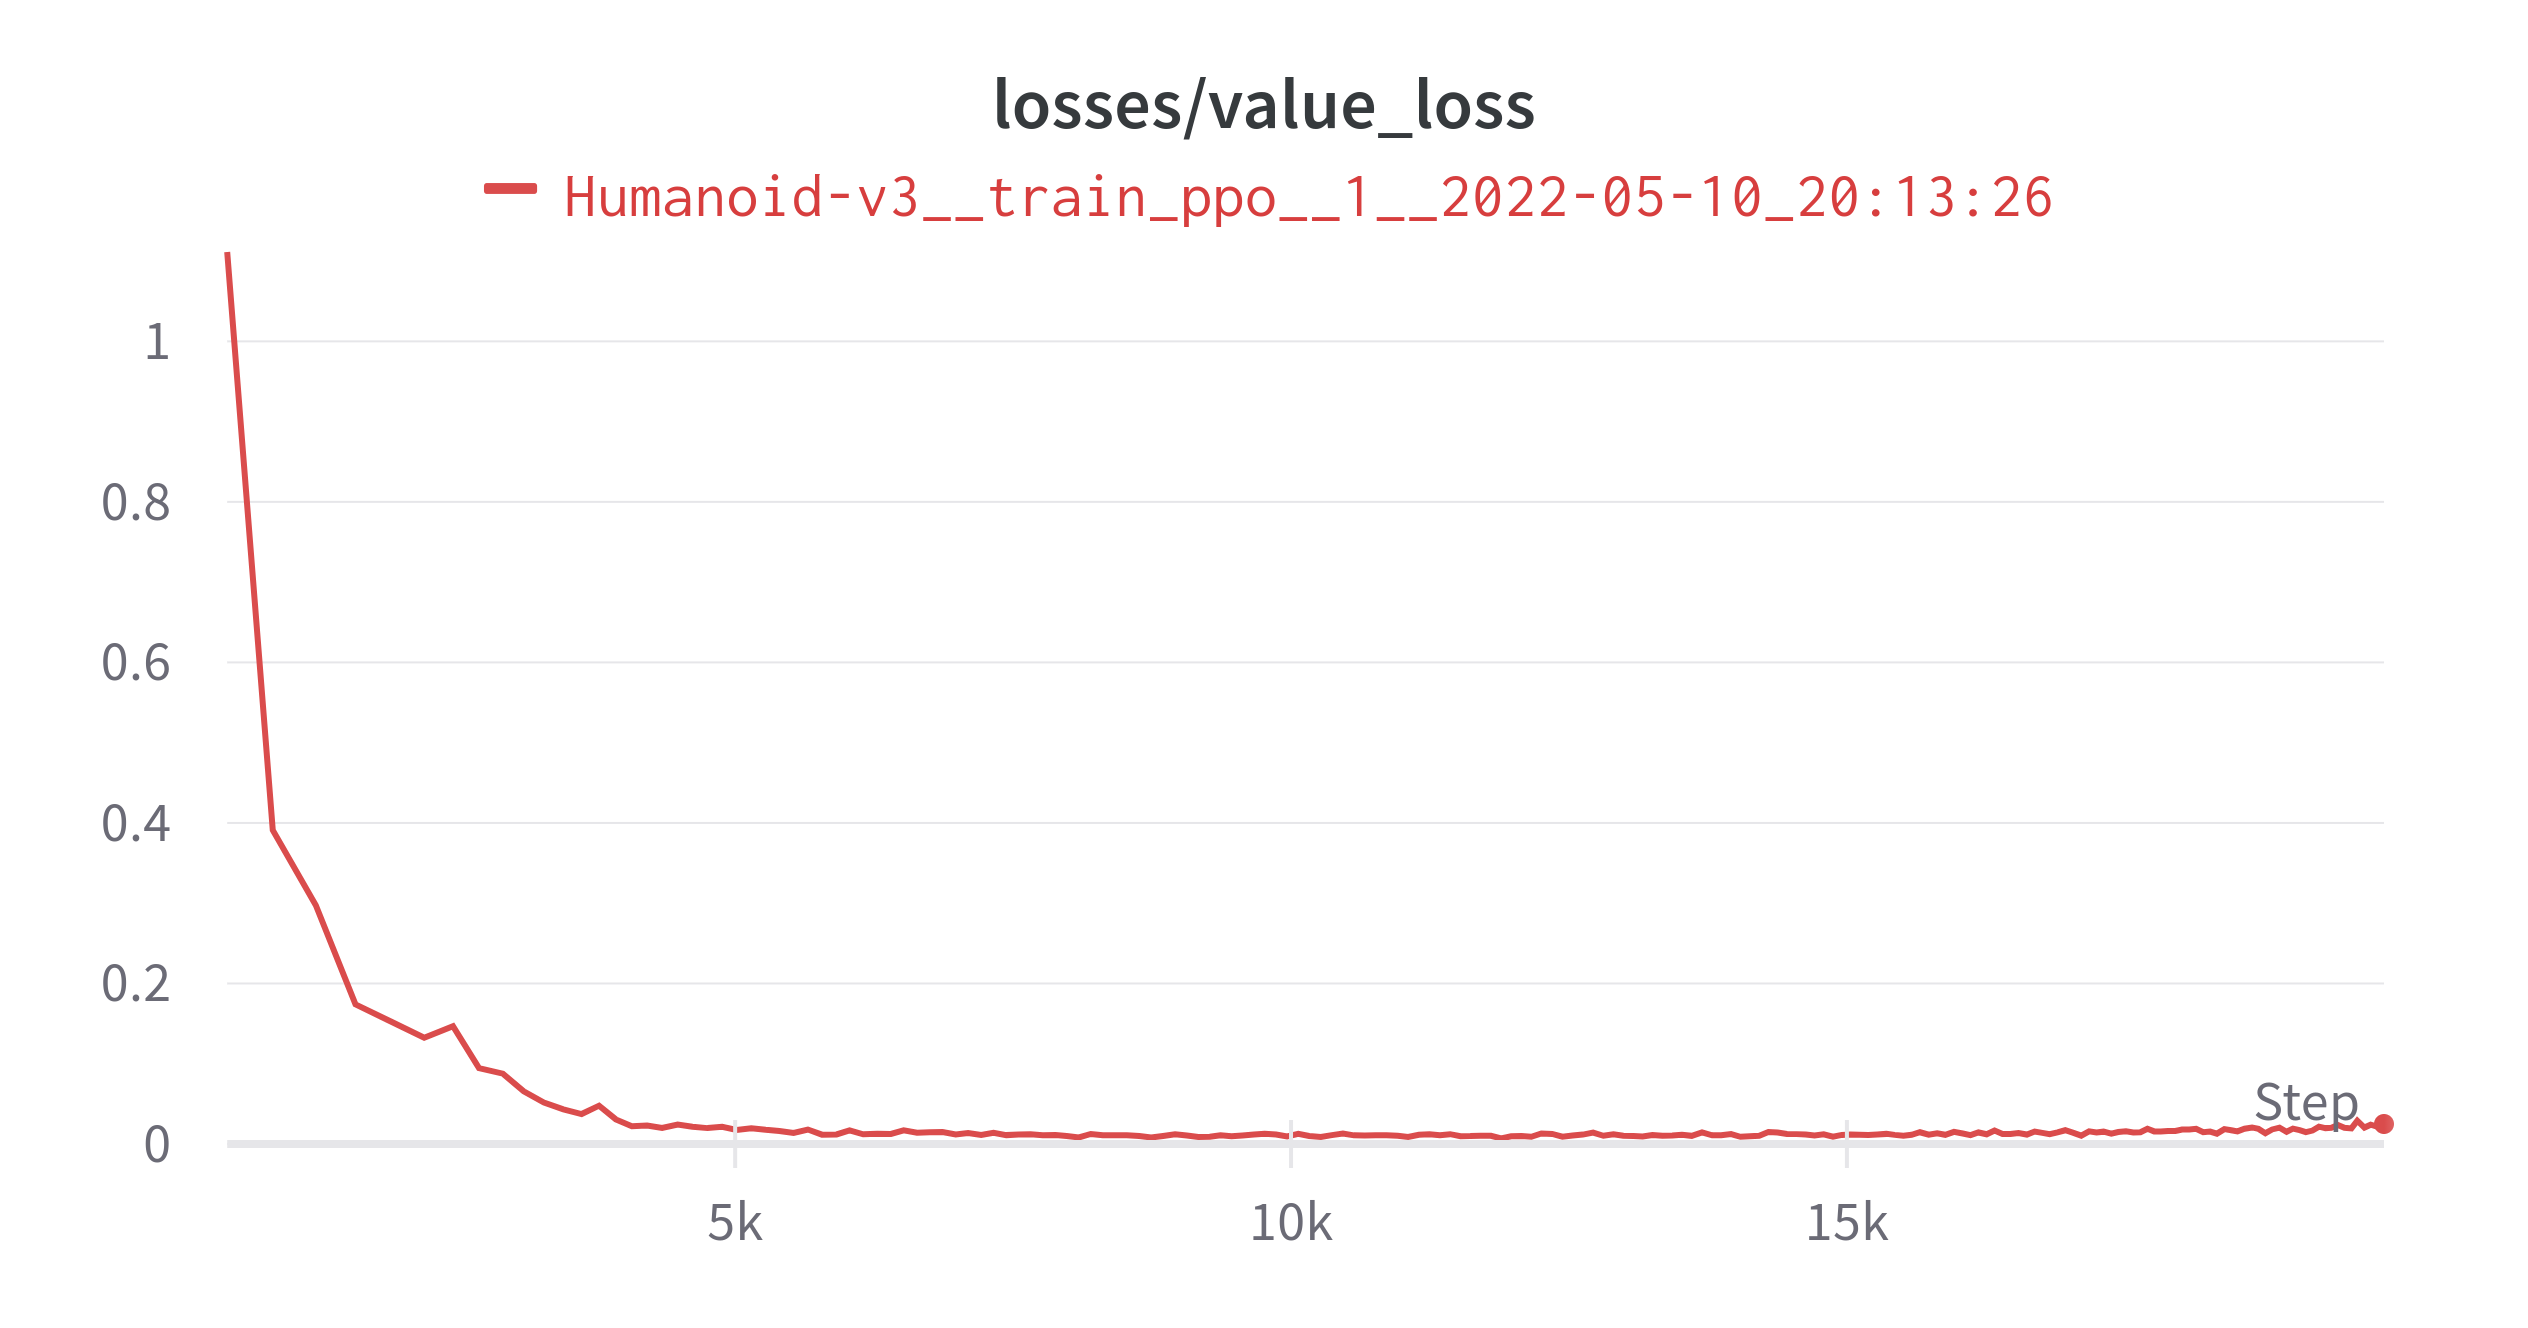
\includegraphics[width=\textwidth]{humanoid_value_loss.png}
            \caption{Value loss on Humanoid-v3}
            \label{fig:imagenet1k}
        \end{minipage}
    \end{figure}
\end{frame}

% Import bibliography from file sample.bib
\begin{frame}{References}
\bibliographystyle{plainnat}
\bibliography{sample}
\end{frame}

\end{document}